%%begin_custom_header
\documentclass[11pt]{article}	% RECOMB: "at least 11 point font size on U.S. standard 8 1/2 by 11 inch paper with no less than one inch margin all around."				
\usepackage[utf8]{inputenc}   % umlauts etc.
\usepackage[english]{babel}
\usepackage [autostyle, english = american]{csquotes}
\MakeOuterQuote{"}
\usepackage{hyperref}
\usepackage{array}
% ----------------------------------
\usepackage[backend=biber,style=nature,sorting=none,url=false]{biblatex}
% url = false. There are also isbn, doi etc., similar options. 
\addbibresource{/Users/mohammedalshamrani/Downloads/School/Waldispul/Publishing/z-misc/zotero-library/my_library.bib}
% ----------------------------------
% Citation style 	biblatex stylename
% ----------------------------------
% 	ACS				chem-acs
% 	AIP				phys (*)
% 	Natur			nature
% 	Science			science
% 	IEEE			ieee
% 	Chicago			chicago-authordate
% 	MLA				mla
% 	APA				apa
% ----------------------------------
% sorting options:
% ----------------------------------
%	nty 		Sort by name, title, year.
%	nyt 		Sort by name, year, title.
%	nyvt 		Sort by name, year, volume, title.
%	anyt 		Sort by alphabetic label, name, year, title.
%	anyvt 		Sort by alphabetic label, name, year, volume, title.
%	ynt 		Sort by year, name, title.
%	ydnt 		Sort by year (descending), name, title.
%	none 		Do not sort at all. All entries are processed in citation order.
% ----------------------------------
\newcommand{\harpoon}{\overset{\rightharpoonup}}
\newtheorem{theorem}{Theorem}
\usepackage{verbatim} % multiline comment
\usepackage{graphicx}
\graphicspath{{/Users/mohammedalshamrani/Downloads/School/Waldispul/Publishing/Paper_04/fig/}}
\setlength\fboxsep{0pt} % figure border padding
\setlength\fboxrule{1pt} % figure outline
\usepackage[fleqn]{amsmath}  % also \documentclass[fleqn]{article}
\usepackage[margin=1in]{geometry}
\abovedisplayskip=0pt
\abovedisplayshortskip=0pt
\belowdisplayskip=0pt
\belowdisplayshortskip=0pt
\setlength{\mathindent}{0pt}
\usepackage{amsfonts} % for R (real numbers)
\usepackage{float}
\usepackage[font=scriptsize,labelfont=bf]{caption}

\usepackage[percent]{overpic}
\usepackage[export]{adjustbox}
% ----------------------------------
%Squeezing the Vertical White Space
%http://www.terminally-incoherent.com/blog/2007/09/19/latex-squeezing-the-vertical-white-space/
% 	THIS FIXES THE PROBLEM OF SUBSECTIONS STARTING IN A NEW PAGE
\setlength{\parskip}{0pt}
\setlength{\parsep}{10pt}
\setlength{\headsep}{0pt}
\setlength{\topskip}{0pt}
\setlength{\topmargin}{0pt}
\setlength{\topsep}{0pt}
\setlength{\partopsep}{10pt}
\usepackage[compact]{titlesec}
\titlespacing{\section}{0pt}{*2}{*2} % {left margin} {above-skip} {below-kip} , The * notation replaces the formal notation using plus/minus and etc. 
\titlespacing{\subsection}{0pt}{*1}{*1}
\titlespacing{\subsubsection}{0pt}{*1}{*1}
% ----------------------------------
\newenvironment{absolutelynopagebreak}
  {\par\nobreak\vfil\penalty0\vfilneg
   \vtop\bgroup}
  {\par\xdef\tpd{\the\prevdepth}\egroup
   \prevdepth=\tpd}
% ----------------------------------
\newcommand{\bfl}{\begin{flushleft}}
\newcommand{\efl}{\end{flushleft}}
\newcommand{\mys }{\hspace{0.1cm}}
\newcommand{\figfont}{\footnotesize}

%begin_custom_header
%\usepackage[backend=biber]{biblatex}
%end_custom_header

%\begin{document}
%begin_custom_content
%\newpage
\section{Approach} \label{approach}	
\subsection{Evolutionary Pressure}		
%We approached the issue from a computational complexity perspective in contrast to previous studies that have been rooted
%in statistical physics. 
A biological network of $n$ genes $(g_1, g_2,\dots, g_n)$ can be represent as an adjacency matrix 
$M=\big [m_{jk}\big ]$, $1\leq j,k\leq n$ where $m_{jk} = +1, -1,\text{or } 0$ implies, respectively,  
that $g_j$ promotes, inhibits, or doesn't interact with $g_k$. At a given point in evolutionary time,
some interactions may become detrimental to the overall fitness of the organism: $g_j$ promotes (inhibits) $g_k$ when the latter should
in fact be inhibited(promoted). Conversely, some interactions can become critically advantageous: $g_j$ promotes (inhibits) $g_k$ when the latter should
indeed be promoted (inhibited). 
Let matrix $A=\big [a_{jk}\big ]$ represent a hypothetical "ideal" regulatory state, such that 
$a_{jk}\in\{+1,-1\}$ if $m_{jk}\neq 0$ and $a_{jk}=0$ otherwise. We refer to $A$ as an "Oracle advice" (OA) on the network. 
While $m_{jk}\neq 0$ describes what the effect of $g_j$ 
on $g_k$ actually is, $a_{jk}$ describes what that effect should \textit{ideally} be. A beneficial (detrimental) interaction
is one where $m_{jk} \times a_{jk} = 1 $ $(m_{jk}\times a_{jk}=-1)$. In other words, an interaction is beneficial (detrimental)
if it is in agreement (disagreement) with what the Oracle says that interaction should ideally be. 
Assume for example that $g_j$ promotes $g_k$, i.e. $m_{jk}=+1$, 
but the OA says that interaction should ideally be inhibitory instead, i.e. $a_{jk}=-1$, then $m_{jk}\times a_{jk}=-1$ implies
the real disagrees with the ideal and the interaction is deemed detrimental. 

 \begin{figure*}[h]
		\centering
		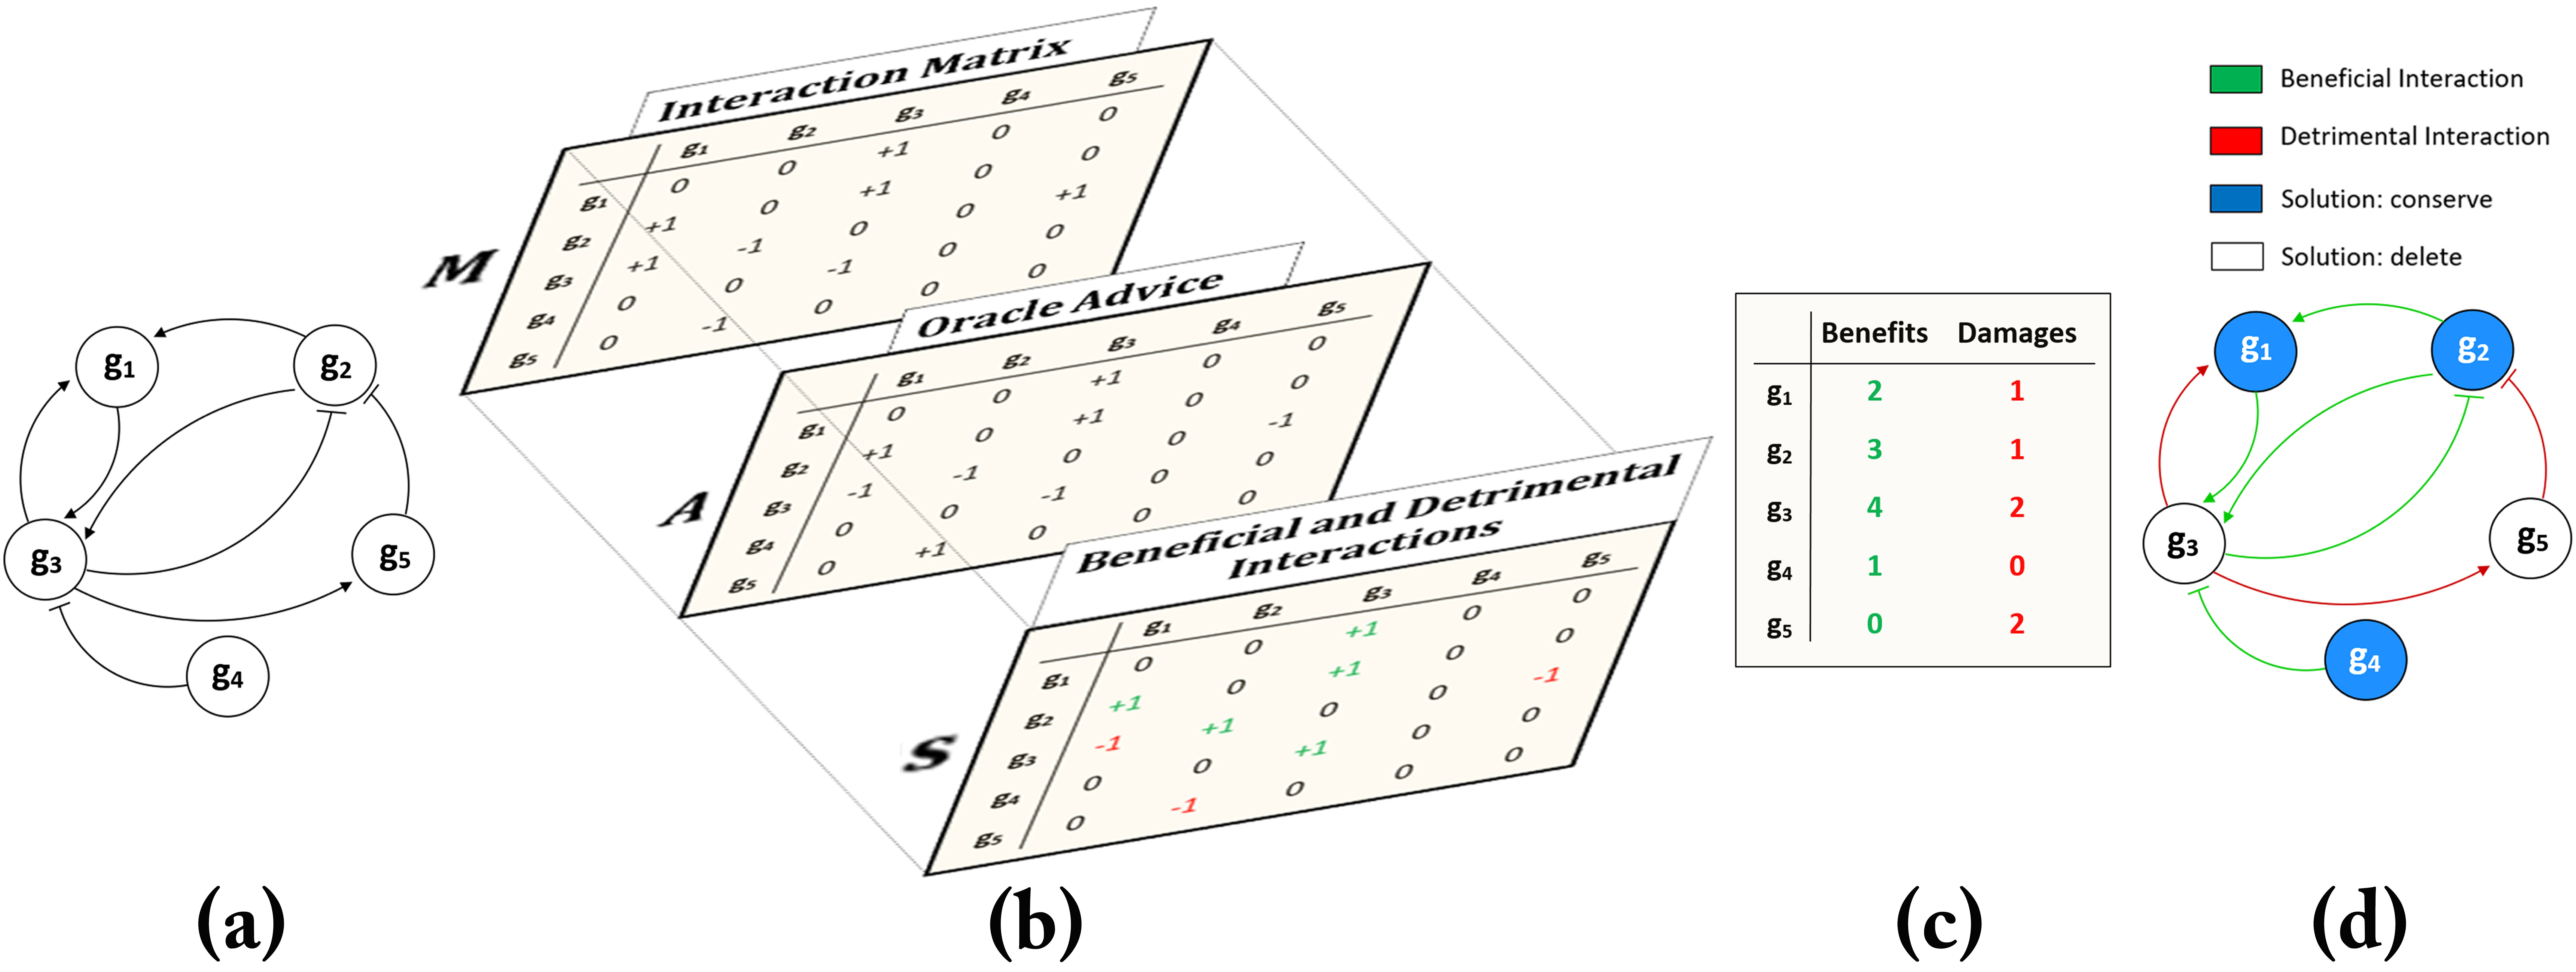
\includegraphics[width=1.0\textwidth]{/intro/photoshop/bigger_matrices.jpg} % original width= 42.65cm,  height = 19.86cm
		\caption{The network evolution problem. (a) A hypothetical  molecular interaction network of five genes $g_1 \dots g_5$ with 
		some inhibitory or promotional interactions (bar- and arrow-terminated edges, respectively). 
		(b) An equivalent representation of the network as an adjacency matrix ($M$). An Oracle advice ($A$) matrix indicates what the interactions in $M$ should 
		ideally be. 
		For example the promotional interaction from $g_1$ to $g_3$ (from $g_3$ to $g_5$) is in agreement (disagreement) with what the 
		Oracle says that interaction should be. Beneficial (in agreement) and detrimental (in disagreement) interactions are 
		shown in the bottom matrix $S$ in which $s_{jk}$ obtained by multiplying each $m_{jk}$ in $M$ with $a_{jk}$ in $A$. (c) Each gene $g_j$ in the network is 
		assigned a benefit (damage) value = the sum of beneficial (detrimental) interactions it projects onto 
		(out-edge, adding absolute values along along row $j$ in $S$) or attracts from (in-edge, adding absolute values along along column $j$ in $S$) other genes. 
		(d) Genes $g_4$, $g_5$ are unambiguous (totally beneficial, i.e. damage=0, or totally detrimental, i.e. benefit=0), while $g_1,g_2$ and $g_3$ 
		are ambiguous (having both non-zero benefit/damage scores). Assuming a threshold 2 tolerable detrimental interactions, the optimal evolutionary trajectory would be to conserve $g_1$,$g_2$ and $g_4$ and delete $g_3$ and $g_5$. }
\label{intro_figure}
\end{figure*}	
The benefit (damage)
score of each gene $g_j$, given an OA, is the sum of beneficial (detrimental) interactions that $g_j$ is
\textit{projecting} onto (out-edges) or \textit{attracting} from (in-edges) other genes. More precisely, the benefit score of $g_j$ is defined as:

 $b_j = \sum\limits_{k=1}^{n} m_{jk} \oplus a_{jk} \hspace{0.1cm}+\hspace{0.1cm} \sum\limits_{k=1}^{n} m_{kj} \oplus a_{kj} \quad\textrm{where:}$ 
 
 $\hspace{2cm}m_{xy} \oplus a_{xy}  =	\scriptscriptstyle{\begin{cases}	% in math mode, use scriptstyle/scriptscriptstyle, not small/tiny
											1 & \quad\textrm{if}\quad m_{xy} \times a_{xy} >0 \\
											0 & \quad\textrm{otherwise} 
									\end{cases}	
									}$
 
\vspace{.5cm}
and similarly the damage score is:
\vspace{.5cm}

$d_j = \sum\limits_{k=1}^{n} m_{jk} \ominus a_{jk} \hspace{0.1cm}+\hspace{0.1cm} \sum\limits_{k=1}^{n} m_{kj} \ominus a_{kj} \quad\textrm{where:}$ 

$\hspace{2cm}m_{xy} \ominus a_{xy}  = \scriptscriptstyle{\begin{cases}	% in math mode, use scriptstyle/scriptscriptstyle, not small/tiny
											1 & \quad\textrm{if}\quad m_{xy} \times a_{xy} < 0 \\
											0 & \quad\textrm{otherwise} 
									\end{cases}	
									}$

\vspace{.5cm}
An organism is clearly better off conserving a gene $g_j$ if its benefit $b_j\neq 0$  and damage $d_j=0$,
and deleting $g_j$ if $d_j\neq 0$ and $b_j=0$. We refer to such genes as \textit{unambiguous}. 
Clearly a degree-1 leaf gene $g_k$ (i.e. it only interacts with one other gene) is always 
unambiguous. A degree-2 $g_k$ can have one of four possible ($b_k$,$d_k$) values: 00, 01, 10, 11 with each digit representing an 
interaction (edge) and 0 or 1 implying the interaction is beneficial or detrimental, respectively, and as such $g_k$ has a 50\%
chance of being unambiguous under a random OA (i.e. equal likelihood of an interaction being deemed beneficial or detrimental by the Oracle).
As the degree $d$ of $g_k$ increases linearly, the probability of it being unambiguous under some OA decreases exponentially (namely,  $prob. = 2^{1-d}$). The network evolution problem (NEP) is that of defining the following function $f$: 

\begin{align*}
\scriptsize {f:\boldsymbol{G}  \rightarrow \{0,1\} \mys \textrm{maximizing} \mys  \sum\limits_{j=1}^{n} f(g_j)\times b_j \mys\mys\textrm{s.t.} \mys\mys \Bigg(  \sum\limits_{j=1}^{n} f(g_j)\times d_j  \Bigg)  \leq \boldsymbol{t} }
\end{align*}

	\begin{table}[t] %h:here, t:top of page, b:bottom of page, more: http://tex.stackexchange.com/questions/35125/how-to-use-the-placement-options-t-h-with-figures
		%\setlength\arrayrulewidth{.1pt}\arrayrulecolor[HTML]{0a84f7} %https://en.wikibooks.org/wiki/LaTeX/Colors#Adding_the_color_package
		\scriptsize %\small \tiny, \scriptsize, \footnotesize, \small, \normalsize, \large, \Large, \LARGE, \huge, and \Huge.
			\setlength\cellspacetoplimit{4pt} % padding in table cells
			\setlength\cellspacebottomlimit{4pt} %padding in table cells
			\begin{tabular}{c|c}  % http://tex.stackexchange.com/questions/302960/modify-arraystretch-for-a-single-row-in-table
				\hline
					BN & Biological Network
				\\[.01cm] \hline
					mLmH & Majority-leaves Minority-hubs topology
				\\[.01cm] \hline
					OA & Oracle Advice
				\\[.01cm] \hline
					NEP & Network Evolution Problem
				\\[.01cm] \hline
				    RVnRS & Random Variation non-Random Selection
				\\[.01cm] \hline
			\end{tabular}
			\caption{Abbreviations}
			\label{abbrev}	
	\end{table}

NEP has previously been proved NP-hard \cite{atiia_computational_2017-1}. Figure \ref{intro_figure} (a) shows a hypothetical small interaction network of 5 genes, 
with promotional and inhibitory interactions denoted by arrows and bars, respectively. The network can equivalently be represented as an (adjacency) 
interaction matrix $M$ (top matrix in Figure \ref{intro_figure} (b)) where +1, -1 signify promotional, inhibitory interaction, respectively 
(notice $m_{jk}$=0  when no interaction exists 
between $g_j$ and $g_k$). Against a hypothetical OA matrix $A$ (middle matrix in Figure \ref{intro_figure} (b)), where $a_{jk}\neq 0$ indicates 
what the interaction  $m_{jk}\neq 0$ should ideally be, an interaction is deemed beneficial or detrimental (bottom matrix in Figure \ref{intro_figure} (b)) 
when $m_{jk}$ and $a_{jk}$ are in agreement  
(i.e. $m_{jk}\times a_{jk}=1$) or disagreement (i.e. $m_{jk}\times a_{jk}=-1$), respectively. 
The benefit (damage) score of $g_j$ is the sum of beneficial (detrimental) interactions it is projecting onto (adding up absolute values along row $j$) 
or attracting from (along column $j$) other genes as shown in Figure \ref{intro_figure} (c). 
Genes that have zero benefit or damage score (respectively $g_5$ and $g_4$ in this example) should unambiguously be conserved (deleted). However, among 
genes with non-zero benefit and damage scores, an optimization search is needed to determine the optimal action (conserve and delete) that maximizes 
(minimizes) the overall total number of beneficial (detrimental) interactions. 
Clearly the larger the number of such ambiguous genes, the harder the optimization task would be. Assuming a certain threshold of tolerable detrimental interactions = 2 
for example, the optimal RVnRS trajectory (Figure \ref{intro_figure} (d)) would be one that leads to the conservation of $g_1,g_2$ and $g_4$, and the deletion of $g_3$ and $g_5$. 

%
\subsection{Evolutionary Algorithm}\label{evo_alg}
Evolutionary pressure is simulated on a network by randomly generating OAs on all interactions. An evolutionary algorithm selects for networks that 
on average yield easier instances of the optimization problem. Instance difficulty is measured by (1) the percentage of genes that are unambiguous 
(benefit and/or damage = 0) and (2) the effective total benefits that are contributed by conserved genes in an optimal solution. Networks whose 
instances are easiest are considered fit, and a new generation of offspring networks are bred from the top performing networks. Offspring 
population are mutated before the next round of OA generation and instance evaluation starts. 
Figure \ref{workflow} depicts the workflow of the algorithm. Individuals in the population are BNs, represented by their interaction matrix $M$. 
Individuals begin with either an empty network or one with randomly assigned edges.
 Mutation  modifies connectivity between nodes by random edge reassignment to two randomly selected nodes, or by
 adding nodes and edges in simulations where network growth occurs. After mutation, the fitness of each network in the population is 
 assessed based on the computational 
ease of the NEP instances that result from applying repeated evolutionary pressure (multiple OAs) on the network.
 Exact replicas are generated from the fittest 10\% of the networks to create the next
population networks. %Over many generations networks adept at producing easier instances of NEP are selected for. 
For a network of $N$ nodes, the unambiguity metric $U$ emphasizes sparsely connected nodes and is defined as the ratio of unambiguous nodes relative to 
the total number of nodes: 

\begin{align*}
U=\frac{|\{g_i:b_i=0|d_i=0\}|}{N}
\end{align*}

The solution vector to an NEP instance is a sequence $(s_1, s_2, .., s_k)$ where $s_i\in\{0,1\}$ 
and $s_i=1 \mys (s_i=0)$ implies "conserve" ("delete").
Accumulated benefits in an NEP instance's optimal solution is a multi-set $B=\{b_i: s_i=1\}$, and the 
effective accumulated benefits $B_e=sum(set(B))$ (i.e. $B_e$ is $B$ normalized by the number of genes it takes 
to contribute a certain benefit value). For example, with $B1=\{1,1,1,2\}$ and $B2=\{2,3\}$, $sum(B1)=sum(B2)$,  but $B1_e=3$ while $B2_e=5$. 
$B_e$ reflects the effort (no. of genes conserved) needed to achieve a certain benefit. Generally, with
a gene of degree $d$ and assuming all its in- and out-edges are in agreement with the OA (i.e. a totally
beneficial gene), it would single-handedly contribute $|d|$ to $B_e$. In the opposite extreme, if such a gene were broken into $n$ specialty genes with degrees
$(d_1, d_2.., d_n), d_i=1 \forall i$, then $B_e$ reduces down to $1$  ($(d_1 + d_2\dots d_n)\div n$) assuming all such genes are beneficial. Let $B_{tot}$ be the total benefit in a given NEP instance (the sum of gained benefits of conserved genes and lost benefits of deleted genes), the fitness of a given NEP instance $S$ is measured as:

\begin{align*}
F(S) = U^\alpha \times \frac {B_e}{B_{tot}}
\end{align*}

where $\alpha\in \approx \mathbb{R}^{+}$. In all simulations, we used $\alpha=2$, which calibrated the opposing effects \cite{kim_positive_2007} 
of the the two selection criteria (instance size in $U$ and effective total benefit in $\frac {B_e}{B_{tot}}$, 
further discussed in \ref{adapt_section} and Figure \ref{adap_fig}). 
The larger a gene's degree is the more ambiguous it can be. Unambiguous genes do not need to be included in the 
computationally costly optimization search and can $a priori$ be deemed beneficial (detrimental) and should therefore be 
conserved (deleted) regardless of the state of other genes. Mutations on unambiguous nodes will have a clear selection 
gradient since they are more likely to be totally beneficial or totally detrimental but not both. 
Although the problem is generally NP-hard, instances with small effective instance size (large number of unambiguous genes) 
are easier to satisfy. 
Clearly a very sparse network results most genes being unambiguous, but it also leads to an explosion of genome size
since more genes are needed to fulfill a function that could have been handled by a single hub gene. 
While $B_e$ measures the ability of a network to capture more benefits with less genes to conserve, 
normalizing it by the total benefits $B_{tot}$ discourages networks that hemorrhage a large number of possible benefits lost to deleted genes.
\begin{figure}[H]
		\centering
		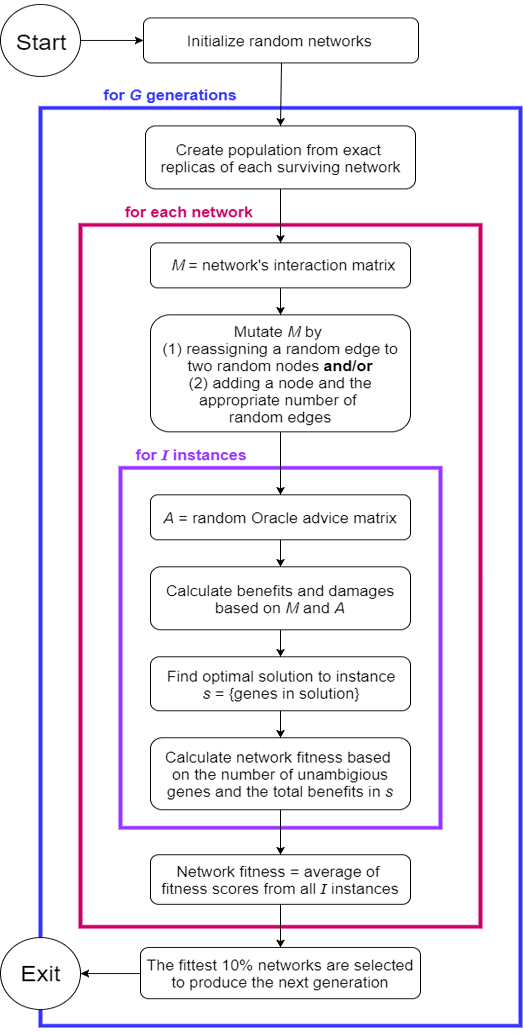
\includegraphics[scale=.42]{workflow/workflow_transparent_2nd_draft.png} % original width= 42.65cm,  height = 19.86cm
		\caption{The algorithmic workflow of the evolutionary algorithm. 
		Simulations begin with empty networks or seed networks that have randomly distributed edges. 
		Each network is randomly mutated by reassigning one edge at each generation and,  
		if growth is allowed, one node is also added along with as many randomly 
		assigned edges as needed to maintain the desired edge:node ratio. 
		An instance of the network evolution problem (NEP) is obtained by generating a random Oracle advice (OA) on all edges in the network. 
		A network's fitness at each instance $S$ is calculated following the $F(S)$ formula (Section \ref{evo_alg}).
		The 10\% of networks with the highest average fitness over all instances are selected to breed a population of networks for the subsequent generation.}
		\label{workflow}
\end{figure}
%	\printbibliography
%\end{document}
%end_custom_content